\documentclass[a4paper,11pt]{article}
\usepackage{amsmath}
\usepackage{wrapfig}
\usepackage{fancyhdr}
\usepackage{graphicx}
\usepackage{url}
\usepackage{float}
\usepackage{amsmath}
\usepackage{amssymb}
\usepackage[margin=1in]{geometry}

%\setlength{\voffset}{-0.5in}
%\setlength{\headsep}{5pt}
\newcommand{\suchthat}{\;\ifnum\currentgrouptype=16 \middle\fi|\;}


%===========---------================
% Author John H Allard
% CMPE 12, Lab #2 Write-up
% October 9th, 2014
%===========---------================


\title{ CMPE 12 Lab Report \# 2 \\[7 in]}
\author{John Allard \\ Steve Lessard \\ Lab Section \#2}
\date{October 16th, 2014}

\begin{document}
\maketitle
\newpage
\tableofcontents
\newpage

%*************************************%
%************* OVERVIEW **************%
%*************************************%

\section{Overview}
This lab, unlike lab \#1, consisted of a single goal. Construct a simple 8-bit ALU using the MultiMedia Logic program. The entire ALU had to be built from scratch, minus a few hints on how to design the input and output layout for the device. This meant that it was completely up to us to determine how we want to divide up, layout, and implement the functionality required by this lab. This also implied that a large portion of our time would be spent planning and prototyping the different parts of the ALU individually before assembling them into one complete unit. \par
Relative to modern ALU's, the one developed in this lab will be a quite simple one. Our ALU is only required to provide two logic functions (AND, NOT), and an ADD function. It would be useful to also include other logic functions like OR, XOR, or NAND, but technically all of these functions can be constructed out of numerous NOT and AND calls, so our ALU is complete. It would also be nice if it could operate on more than 8-bit inputs, but the wiring for a 32-bit or even 16-bit ALU would be much too cumbersome to reasonably accomplish in a bulky simulator like MML. \par  Because this device consists of so many individual components, it has been laid out over 6 consectutive pages in the \texttt{lab2.lgi} document. The list below will inform you what components are on which pages :
\begin{enumerate}
\item Page 1 - Opcode input, operand inputs, input and output displays, state LED's.
\item Page 2 - Source Registers 1 and 2 (SR1 \& SR2), Instruction Register (IR), and first level Opcode decoder.
\item Page 3 - 8-bit Ripple Carry Full-Adder. This takes the data from the SR1 and SR2 registers, the carry-in bit, and produces an 8-bit sum plus a carry out bit.
\item Page 4 - Destination Register (DR), holds the final output of the last operation. This page also contains the logic that controls the output LEDs (P, N, Z, COUT, etc.).
\item Page 5 - ALU Logic Control Section. This section takes the data from SR1 and SR2 and performs the AND and NOT operations on the data. 
\item Page 6 - The final output destination multiplexer. This device takes the results from all of the ALU's functions (AND, ADD, NOT), and determines which of these outputs to route to the destination register (DR) based on the current instruction from the IR. 
\end{enumerate}

When you are simulating my ALU, you will pretty much only need to be looking at the first page. This page contains everything needed to set the inputs and read the outputs. The other 5 pages consist of the underlying circuitry, which will be described in the following 5 or 6 sections of this paper.

%*************************************%
%*********** INPUT/OUTPUT ************%
%*************************************%
\section{Device IO}
This project obviously needs some sort of input and output section to allow the user to properly interact with the ALU. All of the IO components can be found on the first page of the \texttt{lab2.lgi} document, and the layout will look pretty similar to the one presented to us in \texttt{Figure 4} of the \texttt{Lab 2 Instructions PDF}. A high level description of how the user interacts with the ALU is as follows :
\begin{enumerate}
\item Choose an instruction by entering an opcode. 
\item Based on the opcode entered, enter either one or two 8-bit inputs via the HEX keypads. 
\item If needed, set the carry-in bit (only does something during an ADD instruction).
\item Press the `CLOCK' button. 
\item Your output should not be displayed on the output display and the state LEDs should be lit or dim appropriately.
\item Either press the reset button, or go back to the top of this list.
\end{enumerate}

A more in-depth description of the ALLU IO functionality can be found in the two subsections below.

 %\begin{figure}[h!]
  \begin{wrapfigure}{l}{0.72\textwidth}
     %\centering
       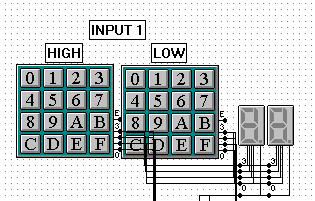
\includegraphics[width=4in]{pictures/8bitinput}
     \caption{8-bit Input Device}
     \label{fig:8bitinput}
  \end{wrapfigure} 

\subsection{Input}
The input for the ALU is relatively simple, and is analagous to many other operations in programming. You need to choose a function to perform, and then give this function some agruments. This function will return a resul that depends on the arguments provided. This is almost exactly how the ALU that I built works, where in our case we have 3 function choices and two input choices. Below is a description of every input that the ALU needs.

   \begin{wrapfigure}{l}{0.65\textwidth}
     %\centering
       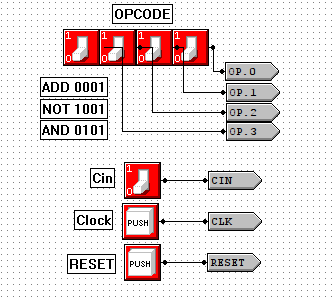
\includegraphics[width=4in]{pictures/opcodeinput}
     \caption{Opcode Input Section}
     \label{fig:opcodeinput}
  \end{wrapfigure} 

  \begin{itemize}
  \item \textbf{One or Two 8-bit Numbers -} These are the two possible arguments that can be used by any function the ALU completes. Both of these inputs are 8-bit numbers, but they individually are entered as a 2-digit HEX number. These numbers are signed using the two's compliment method, so any HIGH hex digit above 7 will have a leading one which will make the number negative. The input for each of these two 8-bit numbers is shown in Figure \ref{fig:8bitinput}

  \item \textbf{4-bit OpCode -} The ALU needs to know which function to perform. Although a 4-bit opcode input could technically specify 16 unique instructions to the ALU, we will only be using three of the available values ( $[1001], [0001], [0101]$ for NOT, ADD, and AND respectively). The opcode is entered by setting 4 switches to either a high or low state, as seen in Figure \ref{fig:opcodeinput}.

  \item \textbf{Carry-In, Clock, and Reset -} The carry-in bit only does something when you also enter the ADD opcode, in this case is sets the carry-in bit to high for the 8-bit full adder. The Clock button allows you to simulate a single clock cycle for the ALU. If you've just set an opcode and an input, you would need to press the clock button to have the inputs propogate through the ALU causing it to generate the correct output. Finally, the reset button just sets all of the memory in the ALU to \texttt{0}.

  \end{itemize}
 \subsection{Output}

  The output for the ALU is also extremely simple, it consists of 2 display screens (one for each HEX digit) and a handful of LED's that give the user more information on the current state of the ALU. The output displays will look identical to the input displays, except they will be labeled output and won't be connected to any keypads. After you complete an operation, the output will be displayed here. If you entered an invalid opcode, you will see an output of \texttt{BC}, which stands for `bad (op)code'. Refer to the previous section for the valid input opcodes. The LED array will tell the user various information about the state of the ALU, for more information, see Figure \ref{fig:resultinfo}

    \begin{figure}[h!]
     \centering
       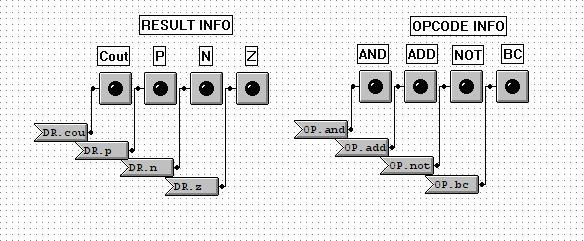
\includegraphics[width=5in]{pictures/resultinfo}
     \caption{LED Output Display}
     \label{fig:resultinfo}
  \end{figure} 



%*************************************%
%************* REGISTERS *************%
%*************************************%

\section{Registers}
The registers are a very important part of the ALU, and there are 4 of them in my implementation. All of the registers in this program are synchronized to the global ALU clock signal, which means a clock cycle is needed to propogate a result into memory. The exception to this is the RESET signal which is connected to every register. This signal is asynchronous and thus will set all bits to \texttt{0} without the need for another clock cycle. All registers are listed below.
  \begin{itemize}
  \item \textbf{Source Registers 1 \& 2 -} 8 bits each. Labeled \texttt{SR1} and \texttt{SR2} in \texttt{lab2.lgi} 
  \item \textbf{Instruction Register} - 4 bits. Labeled \texttt{IR} in \texttt{lab2.lgi}. 
  \item \textbf{Destination Register} - 8 bits. Labeled \texttt{DR} in \texttt{lab2.lgi}
  \end{itemize}

All of these registers are very similar in layout, and with the exception of the instruction register being only 4 bits, they would be nearly identical. A picture of the instruction register can be seen in Figure \ref{fig:instructionregister}

\subsection{Source Registers}
 The ALU needs two registers to store the data it needs to perform computations on, these registers are called the Source Registers. These registers hold the two 8-bit input arguments needed by the ALU. They are 8-bit D-flip-flop registers, with a RESET override line connected to each bit. Every bit is synchronized to the clock signal for the ALU, which means you need a clock cycle to propogate a result into memory. The input to these registers comes from the input keypads on page 1 of \texttt{lab2.lgi}, and the output of these registers is routed to each of the three ALU functions. Both of these registers can be seen on page 2 of the \texttt{lab2.lgi} project.

\subsection{Instruction Register}

   \begin{wrapfigure}{l}{0.68\textwidth}
     %\centering
       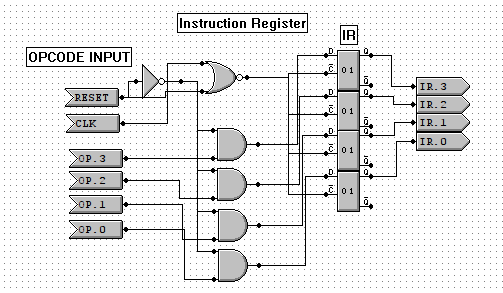
\includegraphics[width=4.2in]{pictures/instructionregister}
     \caption{4-bit Instruction Register}
     \label{fig:instructionregister}
  \end{wrapfigure} 

  The instruction register is very much like the source registers, except it only needs to store 4 bits of information. Technically, since we only are using 3 valid opcodes, we could use as little as two bits for the IR, but having four bits available will allow us to easily add more opcodes in the near future. The instruction register (IR) can be seen in \ref{fig:instructionregister}. It, like the other registers, has the reset line tied to the clock input for each flip-flop, allowing it to be asynchronously reset with a push of the reset button on the first page of the project. 

\subsection{Destination Register}

The final register in that the ALU needs to operate is the Destination Register (DR). This register recieves the final 8-bit result of the last computation performed by the ALU, and stores it for use by the output displays or the user. The final value that is stored inside of this register depends on the opcode entered by the user. This is because all of the functions (NOT, ADD, AND) are computed during each clock cycle, then all of these outputs are routed to a final series of MUX's, which only direct the desired result to the destination register. This register also has a reset line connected to the clock signal, which allows an asynchronous reset.

%*************************************%
%*************** LOGIC ***************%
%*************************************%
\section{ALU Logic}
The logic for this particular ALU was not too difficult to accomplish. This was in part because we are computing every function during every clock cycle, then choosing the appropriate result to route to the DR. This means we don't have to do any complicated signal choosing based on the opcode inside of the arithmetic or logic functions. The two functions that we were instructed to implement were the NOT and AND functions, which are discussed in more detail below.

\subsection{NOT}
The NOT function was extremely simple to implement, and can be seen in Figure \ref{fig:notfunction}. All we do is take each of the 8 bits from the Source Register \#1, route each of these through an inverter gate, and then send the output to the final destination MUX. 

  \begin{figure}[h!]
     \centering
       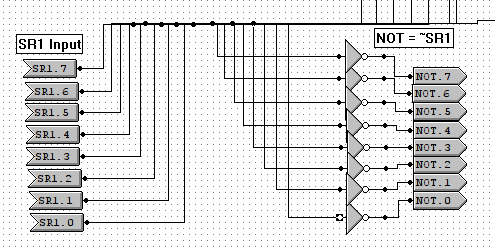
\includegraphics[width=4.7in]{pictures/notfunction}
     \caption{ALU Bitwise NOT Operation}
     \label{fig:notfunction}
  \end{figure} 

\subsection{AND}
The AND function is the only other logical function that needed to be implemented by the ALU. This is a simple 8-bit bitwise AND function that works on the SR1 and SR2 inputs. There is nothing special to see here, I literally just route each corresponding bit from the two source registers to the own 2-input AND gate, then route the output from all of these AND gates to the final destination MUX. Figure \ref{fig:andfunction} shows this AND gate in action. What is interesting is that we could take the output from the AND gate, route it to SR1, then perform a NOT operation on this data. This would be the equivelent of a NAND gate, and since any logical function can be made as a combination of AND gates, our ALU could potentially perform any logical function that works on either one or two 8-bit inputs.

  \begin{figure}[h!]
     %\centering
       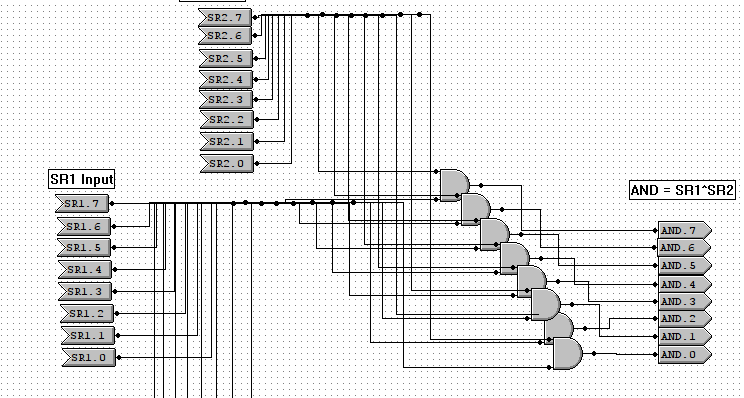
\includegraphics[width=5.4in]{pictures/andfunction}
     \caption{ALU Bitwise AND Operation}
     \label{fig:andfunction}
  \end{figure} 



%*************************************%
%************* Arithmetic ************%
%*************************************%
\section{ALU Arithmetic}
This was one of the more complicated components of the ALU to design and implement. One of the specifications of the ALU was that it needs to be able to add two 8-bit numbers. These numbers are stored in the SR1 and SR2 registers, and the result of the addition is sent to the final destination MUX. The adding function is implemented via a ripple-carry full-adder. This takes the two 8-bit inputs and a carry-in bit, then produces a sum and a carry-out bit. This 8-bit adder consists of 8 cascading full adders, with the carry-out of $S_i$ serving as the carry in for $S_{i_1}$, and the final carry-out bit being sent to an LED that the user can see. An image of how I construct my ripple-carry adder can be seen in Figure \ref{fig:addfunction}. \par
The figure only shows 2 full-adders connected together, the one in the project has 8 of course. The $S$ (sum) bit is generated by the boolean function $S = C_{in} \oplus (A \oplus B)$, which in english states that the sum bit is $1$ only if one of the three inputs has a value of $1$. The carry-out bit is generated with the boolean function $C_{out} = ((A \oplus B) \wedge C_{in}) \vee (A \wedge B)$. The $S_i$ bits (for $ 0 < i < 7$) are sent out to the final destination multiplexer which determines if they are needed or not. The $C_{out}$ bit is send to the LED Logic Controller to be used in determining what LED's to light up after a given operation. 

  \begin{figure}[h!]
     %\centering
       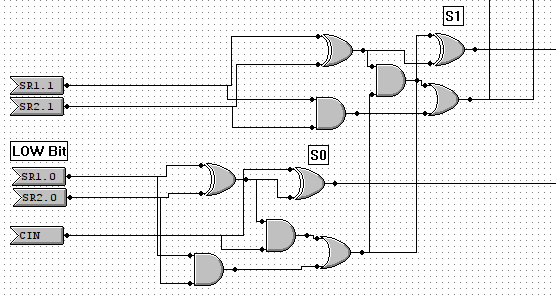
\includegraphics[width=5.4in]{pictures/addfunction}
     \caption{ALU Bitwise ADD Operation}
     \label{fig:addfunction}
  \end{figure} 


%*************************************%
%*********** DATA SELECTION **********%
%*************************************%
\section{Logistics}
This section will explain how I dealt with the problem of moving the data around, including determining the instruction from the opcode, and using that instruction to determine which function output to route to the destination register.

\subsection{Opcode Decoder}
Normally, with a 4-bit opcode, a much more complicated decoder is needed than the one I have in my project. The reason mine is so simple is because we are only using 3 of the possible 16 opcodes, so I only really need to test for those 3 cases. If those three cases all fail, then I know the opcode was invalid and I can set the bad code (BC) bit to let the user know this information. The decoder can be seen in figure \ref{fig:opdecoder}, it takes in 4 bits (\texttt{OP.0} through \texttt{OP.3}) from the instruction register (IR) and turns high one of 4 output lines. The 4 output lines are $[\texttt{AND, ADD, NOT, BC}]$, and have a 1-to-1 mapping to a specific opcode, allowing us to no longer have to decode the binary input when trying to determine which function output to route to the destination register. The simplification that this affect has can be seen in the next subsection.

  \begin{figure}[h!]
     %\centering
       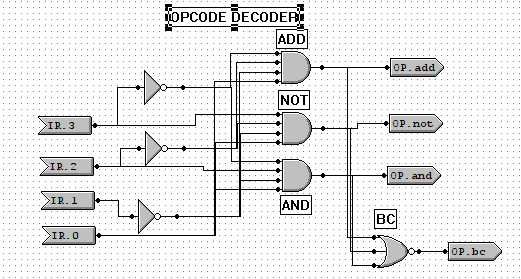
\includegraphics[width=5.4in]{pictures/opdecoder}
     \caption{OpCode Decoder}
     \label{fig:opdecoder}
  \end{figure} 

\subsection{Destination Multiplexer}

   \begin{wrapfigure}{l}{0.68\textwidth}
     %\centering
       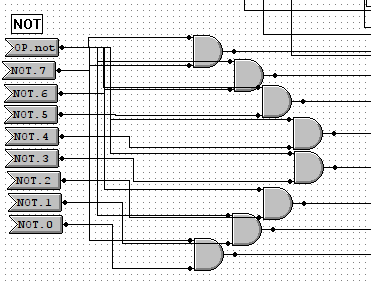
\includegraphics[width=4.2in]{pictures/finalmux1}
     \caption{Final Mux Circuitry Example}
     \label{fig:finalmux1}
  \end{wrapfigure} 


This is a very important part of the ALU, it takes in the output from every function that the ALU can compute (AND, NOT, ADD), and based on the signal set by the opcode decoder, routes one of these 8-bit outputs to the destination register. Because the opcode was already decoded from it's 4-bit binary to form single signal lines, we only have to bitwise AND each bit from each output with the signal line, then OR the outputs for each bit together, finally routing the chosen 8-bits to the destination register. A small example of this can be seen in Figure \ref{fig:finalmux1}. The output from the NOT function is bitwise AND'd with the NOT opcode signal, so if the NOT opcode signal is high, the 8-bits coming from the NOT function pass through while the results from the other functions are blocked. 

%*************************************%
%************** ANALYSIS *************%
%*************************************%



\end{document}